\section{The Diffractometer}

\begin{figure}
	\centering
	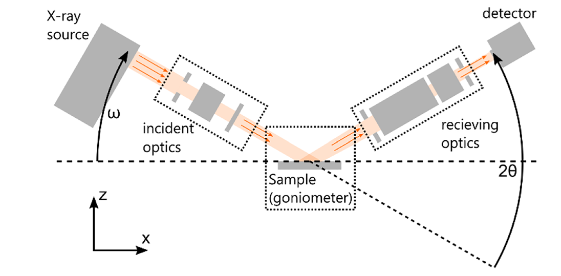
\includegraphics[width=0.6\linewidth]{../assets/xrd_setup.png}
	\caption{XRD Setup}
	\label{fig:xrd_setup}
\end{figure}

A typical XRD Setup is depicted above. An X-Ray Source with a tungsten cathode
and a copper anode generates incident $\ce{Cu}_{\mathrm{K}_{\alpha}}$ x-rays
with a wavelength of $\lambda=\pu{ 1.540592(2) A}$. The beam goes through the XRD
Incident and Receiving Optics|incident optics and hits the sample holder at an angle
$\Omega$. The scattered x-ray beam passes the receiving optics and is detected
by an X-Ray Detector that is mounted on a rocking cantilever. It encloses an angle
of $2\theta$ with the incident beam. The instrument is contained in a radiation
enclosure, controlled by a computer.

The crystal is glued onto the sample holder of a Goniometer. This device can
rotate the sample around the three Euler angles $\Omega$, $\varphi$ and $\chi$.

\subsection{X-Ray Source}

X-rays are produced in an evacuated x-ray tube. Electrons are generated by thermionic
emission of a heated tungsten cathode. As a voltage of 10 to 20 kV is applied
between the heated cathode and a copper anode, the electrons are accelerated towards
the anode. They collide with the anode and ionize the copper atoms. During subsequent
electronic relaxation, a photon is emitted. Its energy depends on the available energy
levels of the material. The strongest radiation originates from the $K$-lines ($K
_{\alpha 1}, K_{\alpha2}, K_{\beta}$). $K_{\alpha}$ radiation is used for measurement
while $K_{\beta}$ is undesirable and therefore often filtered using a monochromator.
Excessive use of a tungsten cathode leads to tungsten contamination on the anode.
This leads to additional peaks in the spectrum.

X-rays are focused on a strip and are passed through a beryllium window as either
point or line spots. It needs to be water-cooled due to the heat generated by
thermionic emission. The tube features a safety shutter which enables manual work
on the beam path or the sample without shutting down the tube.

\subsection{X-Ray Detector}

An x-ray detector converts x-rays into an electrical signal, usually measured in counts
per second (cps). There exists a variety of types, depending on the underlying physics,
for example:

\begin{itemize}
	\item proportional counters

	\item scintillation counters

	\item solid-state detectors Detectors can either measure a pointlike region, a
		line or an area. An important metric is the maximum count rate. By
		overstepping this limit, the detector starts responding non-linearly or even sustains
		damage.
\end{itemize}

\subsection{Incident and Receiving Optics}

A major challenge of the diffraction setup is to condition the divergent x-rays
that leave the source into a parallel beam before it reaches the sample. This conditioning
occurs within the incident beam optics. The procedure is necessary to avoid
divergence errors, as small deviations of the incoming radiation direction smear out
the scattering vector. A suitable condition device is a laterally graded
multilayer mirror. This mirror is designed for a specific wavelength, thus
reducing the unwanted $K_{\beta}$ radiation as well as Bremsstrahlung. It does not
reduce the x-ray intensity significantly. Since the divergence in axial
direction is unaffected by the mirror, it must be constrained through Soller slits.
Installing an axial slit reduces the beam spot size.

To restrict the incoming radiation wavelength around the $K_{\alpha 1}$ peak, a channel-cut
crystal monochromator can be used in the receiving optics. The device consists
of two high-quality single crystal germanium mirrors arranged as depicted above, and
it is defined by the crystal being used, the Miller index of the diffracting
lattice plane, as well as the number of reflections. While the lab instrument
features a 2xGe(220) monochromator, installing one leads to intensity loss. It is
not required in solid-state detector setups as they can select a narrow energy window.
Also installed in the receiving optics are attenuators, which are devices to reduce
the intensity of an x-ray beam. These are vital components for high-intensity
reflections that would otherwise damage the detector, and a thin metal foil placed
in the beam path can be used as an attenuator.

\subsection{Goniometer}

The goniometer can adjust the different angles between x-ray source, sample and x-ray
detector. Diffractometers used for thin film characterization usually feature a
four-axis goniometer. In this setup, the source is installed in a fixed position,
while the sample stage can be rotated through the angles $\varphi$ (inner axis),
$\chi$ (intermediate axis) and $\omega$ (outer axis). Additionally, the position
of the detector can also be set using the angle $2\theta$. Most goniometers can translate
the sample stage in multiple directions.

\subsection{Coordinate Systems}

An XRD experiment features two coordinate systems:

\begin{itemize}
	\item A two-dimensional laboratory frame (red), defined by the Goniometer axes.

	\item The Reciprocal Lattice (blue), which is defined by the crystal lattice.
\end{itemize}

The operations of the goniometer either change the relative position of both coordinate
systems or the scattering vector $\mathbf{q}$.

The laboratory frame coincides with the incidence plane, which is spanned by $\mathbf{k}
_{\mathrm{in}}$ and $\mathbf{k}_{\mathrm{out}}$. The frame is fixed by the
goniometer and does not move with the crystal. Its two basis vectors are defined as:

\begin{itemize}
	\item $q_{\perp}$ - perpendicular to the line where the sample holder plane intersects
		the incidence plane

	\item $q_{\parallel}$ - perpendicular to $q_{\perp}$ and therefore lies in the sample
		holder plane.
\end{itemize}

Two angles $\theta$ and $\Omega$ are used to describe $\mathbf{q}$ within the
laboratory frame and can be set using the goniometer. $2\theta$ is the angle between
$\mathbf{k}_{\mathrm{in}}$ and $\mathbf{k}_{\mathrm{out}}$ and $\Omega$ is the angle
between the sample holder surface and $\mathbf{k}_{\mathrm{in}}$:


The magnitude of $\mathbf{q}$ can be represented using only $\theta$ as:

\[
	\begin{align}
		\lvert \mathbf{q}\rvert^{2} & =\lvert \mathbf{k}_{\mathrm{out}}- \mathbf{k}_{\mathrm{in}}\rvert^{2}=k^{2}+k^{2}-2k^{2}\cos(2\theta)=2k^{2}(1-\cos(2\theta))=4k^{2}\sin^{2}(\theta) \\
		\lvert q \rvert             & =2k \sin(\theta)
	\end{align}
\]
It can also be shown that the angle between the lattice plane perpendicular to
$\mathbf{q}$ and $\mathbf{k}_{\mathrm{out}}$ is $\theta$. Define $\alpha$ as the angle
between $\mathbf{q}$ and $\mathbf{k}_{\mathrm{out}}$:

\[
	\begin{align}
		\mathbf{k}_{\mathrm{out}}\cdot \mathbf{q} & =\mathbf{k}_{\mathrm{out}}\cdot(\mathbf{k}_{\mathrm{out}}-\mathbf{k}_{\mathrm{in}})=k^{2}-k^{2}\cos(2\theta)=2k^{2}\sin^{2}(\theta)            \\
		\cos(\alpha)                              & =\frac{\mathbf{k}_{\mathrm{out}}\cdot \mathbf{q}}{ k \cdot q }=\frac{2k^{2}\sin^{2}(\theta)}{2k^{2}\sin(\theta)}=\sin(\theta)=\cos(90°-\theta)
	\end{align}
\]

$\alpha=90°-\theta$ is the angle between lattice plane normal and $\mathbf{k}_{\mathrm{out}}$
and therefore $\theta$ is the angle between lattice plane and $\mathbf{k}_{\mathrm{out}}$.

To represent $\mathbf{k}_{\mathrm{in}}$ and $\mathbf{k}_{\mathrm{out}}$ using $\theta$
and $\Omega$, note that $\Omega$ is just the negative polar angle of
$\mathbf{k}_{\mathrm{in}}$, and $\mathbf{k}_{\mathrm{out}}$ is obtained by rotating
$\mathbf{k}_{\mathrm{in}}$ by $2\theta$:

\[
	\begin{align}
		\mathbf{k}_{\mathrm{in}}  & = k \begin{pmatrix}\cos(\Omega) \\ -\sin(\Omega)\end{pmatrix}                                                                                                                                                                                       \\
		\mathbf{k}_{\mathrm{out}} & = k \begin{pmatrix}\cos(2 \theta) & -\sin(2\theta) \\ +\sin(2\theta) & \cos(2\theta)\end{pmatrix} \begin{pmatrix}\cos(\Omega) \\ -\sin(\Omega)\end{pmatrix} =k \begin{pmatrix}\cos(2\theta-\Omega) \\ \sin(2\theta-\Omega)\end{pmatrix}             \\
		\mathbf{q}                & =\mathbf{k}_{\mathrm{out}}-\mathbf{k}_{\mathrm{in}}=k \begin{pmatrix}\cos(2\theta-\Omega)-\cos(\Omega) \\ \sin(2\theta-\Omega) + \sin(\Omega)\end{pmatrix} = 2k \sin(\theta) \begin{pmatrix}\sin(\Omega-\theta) \\ \cos(\Omega-\theta)\end{pmatrix}
	\end{align}
\]

This equation also implies $q_{\parallel}/ q_{\perp}=\tan(\Omega-\theta)$. These
two angles act on the system in different ways. Changing $\theta$ only modifies the
scattering vector $\mathbf{q}$ through the relations above. It leaves the
orientation of the laboratory and crystallographic frames untouched. Changing $\Omega$
rotates the laboratory frame as well as the reciprocal lattice by the same amount,
so that the reciprocal lattice does not move relative to the laboratory frame. Because
the laboratory frame itself has turned, the coordinates of the scattering vector
change accordingly, as captured by the formula for $\mathbf{q}$.

The reciprocal lattice orientation depends on the direct lattice, and therefore on
the position of the crystal with respect to the sample holder. As $\theta$ only
moves the detector and $\Omega$ moves both the laboratory frame and the
reciprocal lattice, neither angle changes the relative position between the two coordinate
systems.

The two angles that operate on the reciprocal lattice, $\chi$ and $\varphi$, share
an important property: neither of them rotates the laboratory frame. Instead,
they rotate only the reciprocal lattice, which changes its orientation \emph{relative
to} the laboratory frame.
